\section{Motivation}
\begin{comment}
\subsection{Why centralization?}
\begin{itemize}
	\item Like in traditional SDN argument, a centralized control platform enables the development of flexible, reliable and feature-richer network control plane.
	\item Centralization enables global coordination of resources to optimize for complex application goal. Use example.
	\item Centralization enables better recovery and convergence in disruptive/congested networks. Use example.
\end{itemize}

\subsection{Why not fully centralized?}
\begin{itemize}
	\item Longer propagation delay than in LAN/WAN. \jc{need measurement data to support this.}
	\item Long delay to get a converged network view under large-area disruption/congestion. \jc{need measurement data to support this.}
\end{itemize}

\subsection{Two level control plane design}
Present our design of control plane that runs both in local node and controller.
\end{comment}





\begin{figure}[t]
\centering
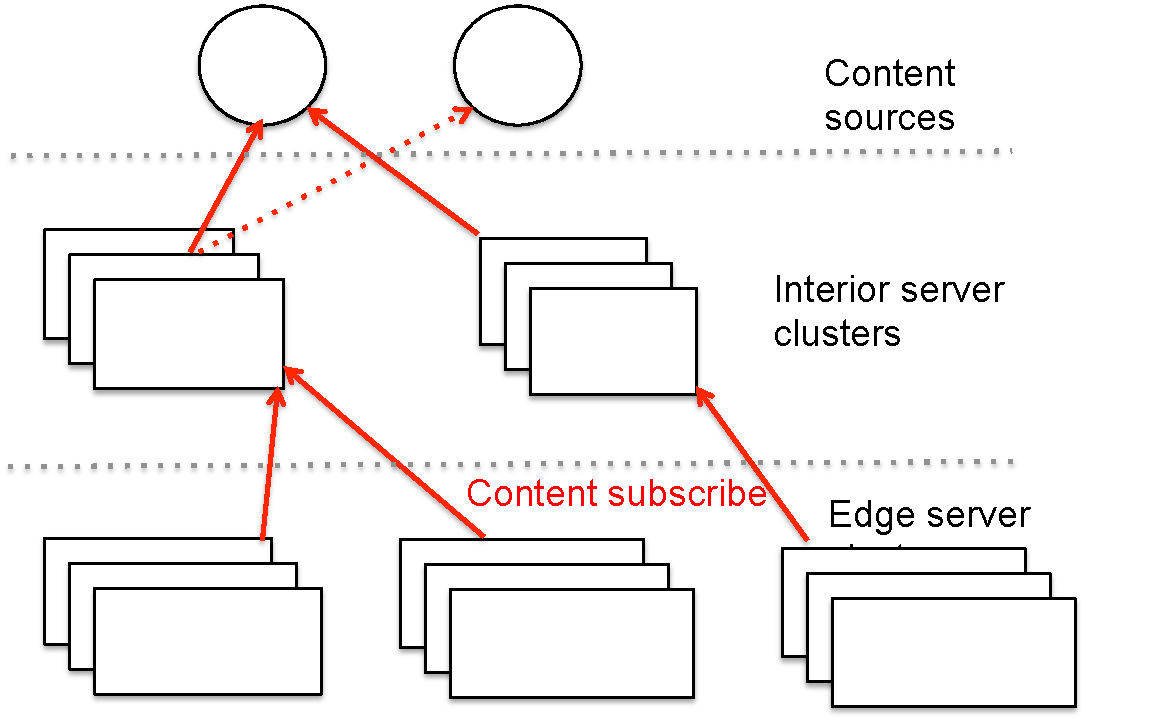
\includegraphics[width=0.90\columnwidth]{figures/cdn}
\caption{Structure of live content distribution in a CDN~\cite{akamai-live}.}
\label{fig:cdn}
\end{figure}

\captionsetup{font=small}

\begin{figure}[t]
\centering
\begin{minipage}[b]{0.32\columnwidth}
  \centering
  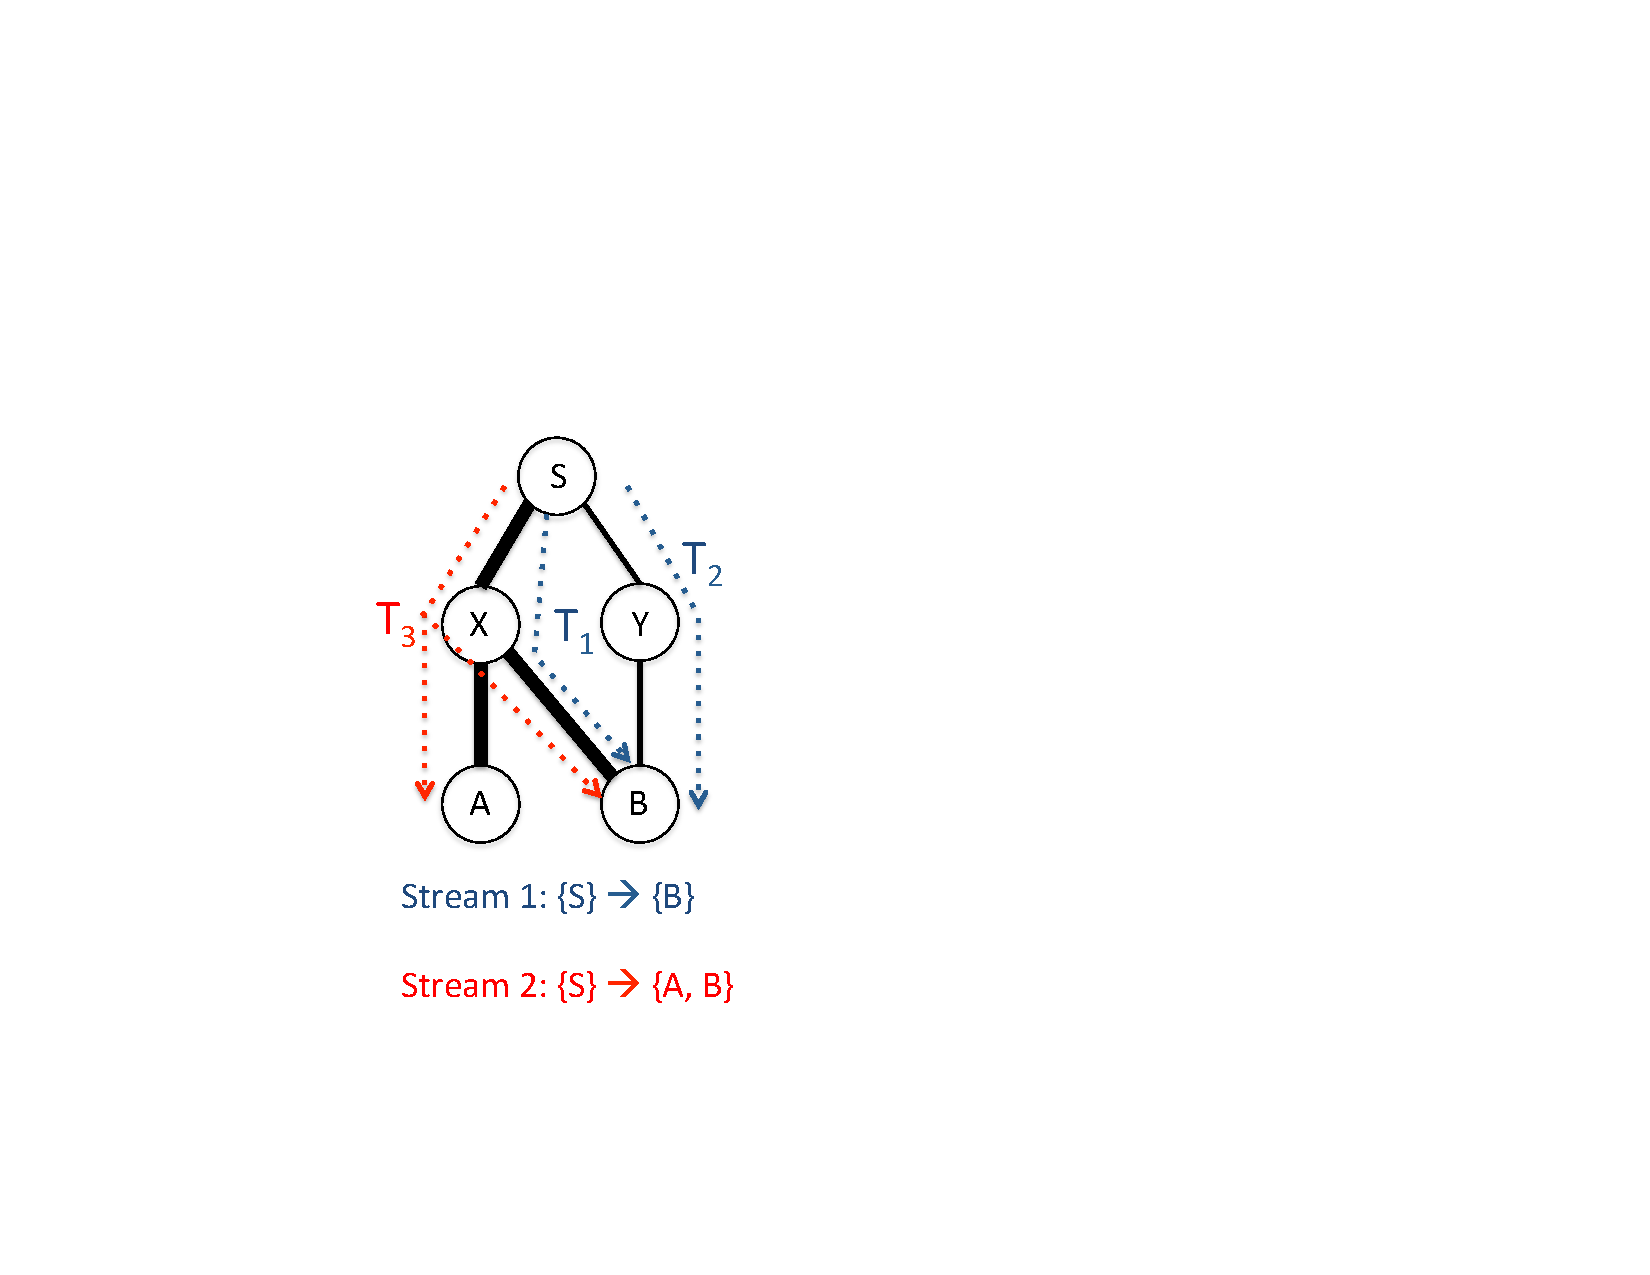
\includegraphics[scale=.40]{figures/toy-alltrees}
  \caption{\\Example Scenario}
  \label{fig:toy-alltrees}
\end{minipage}
\begin{minipage}[b]{0.32\columnwidth}
  \centering
  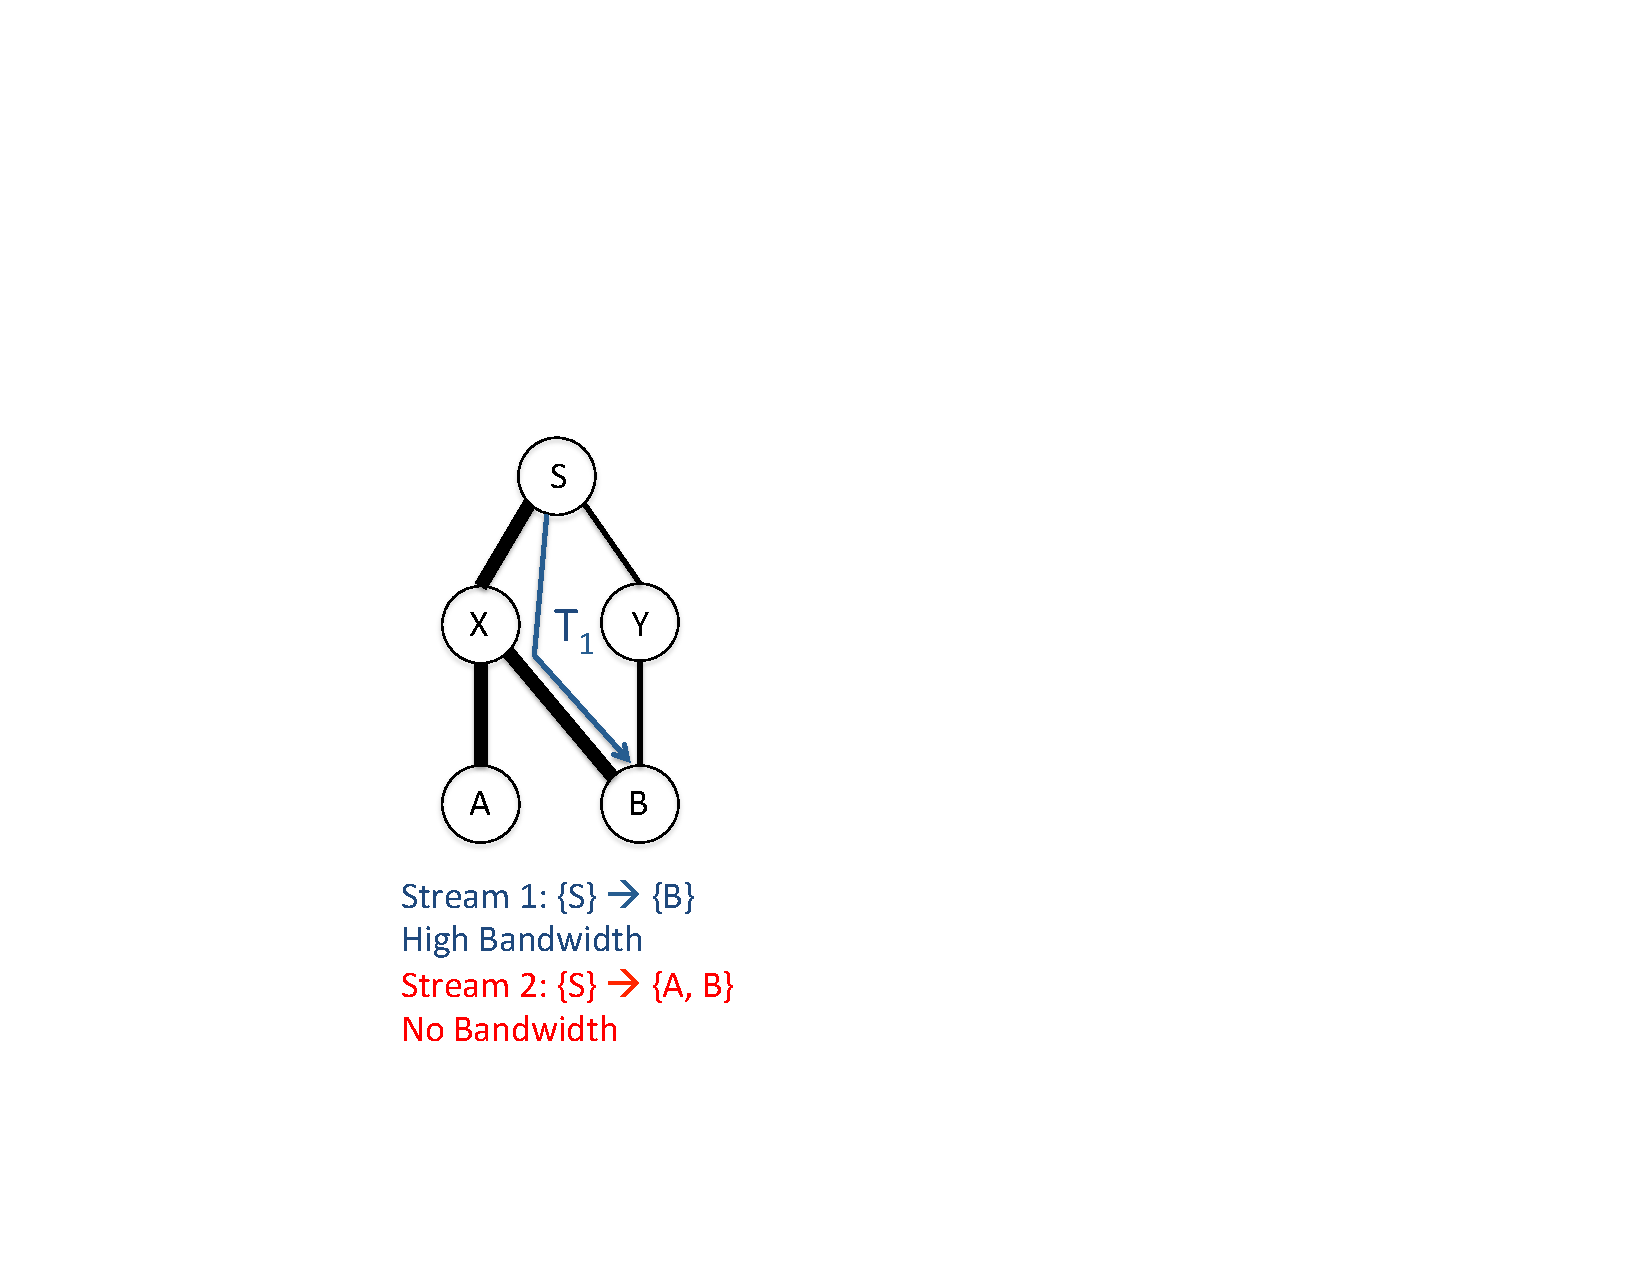
\includegraphics[scale=.40]{figures/toy-current}
  \caption{\\Current CDN}
  \label{fig:toy-current}
\end{minipage}
\begin{minipage}[b]{0.32\columnwidth}
  \centering
  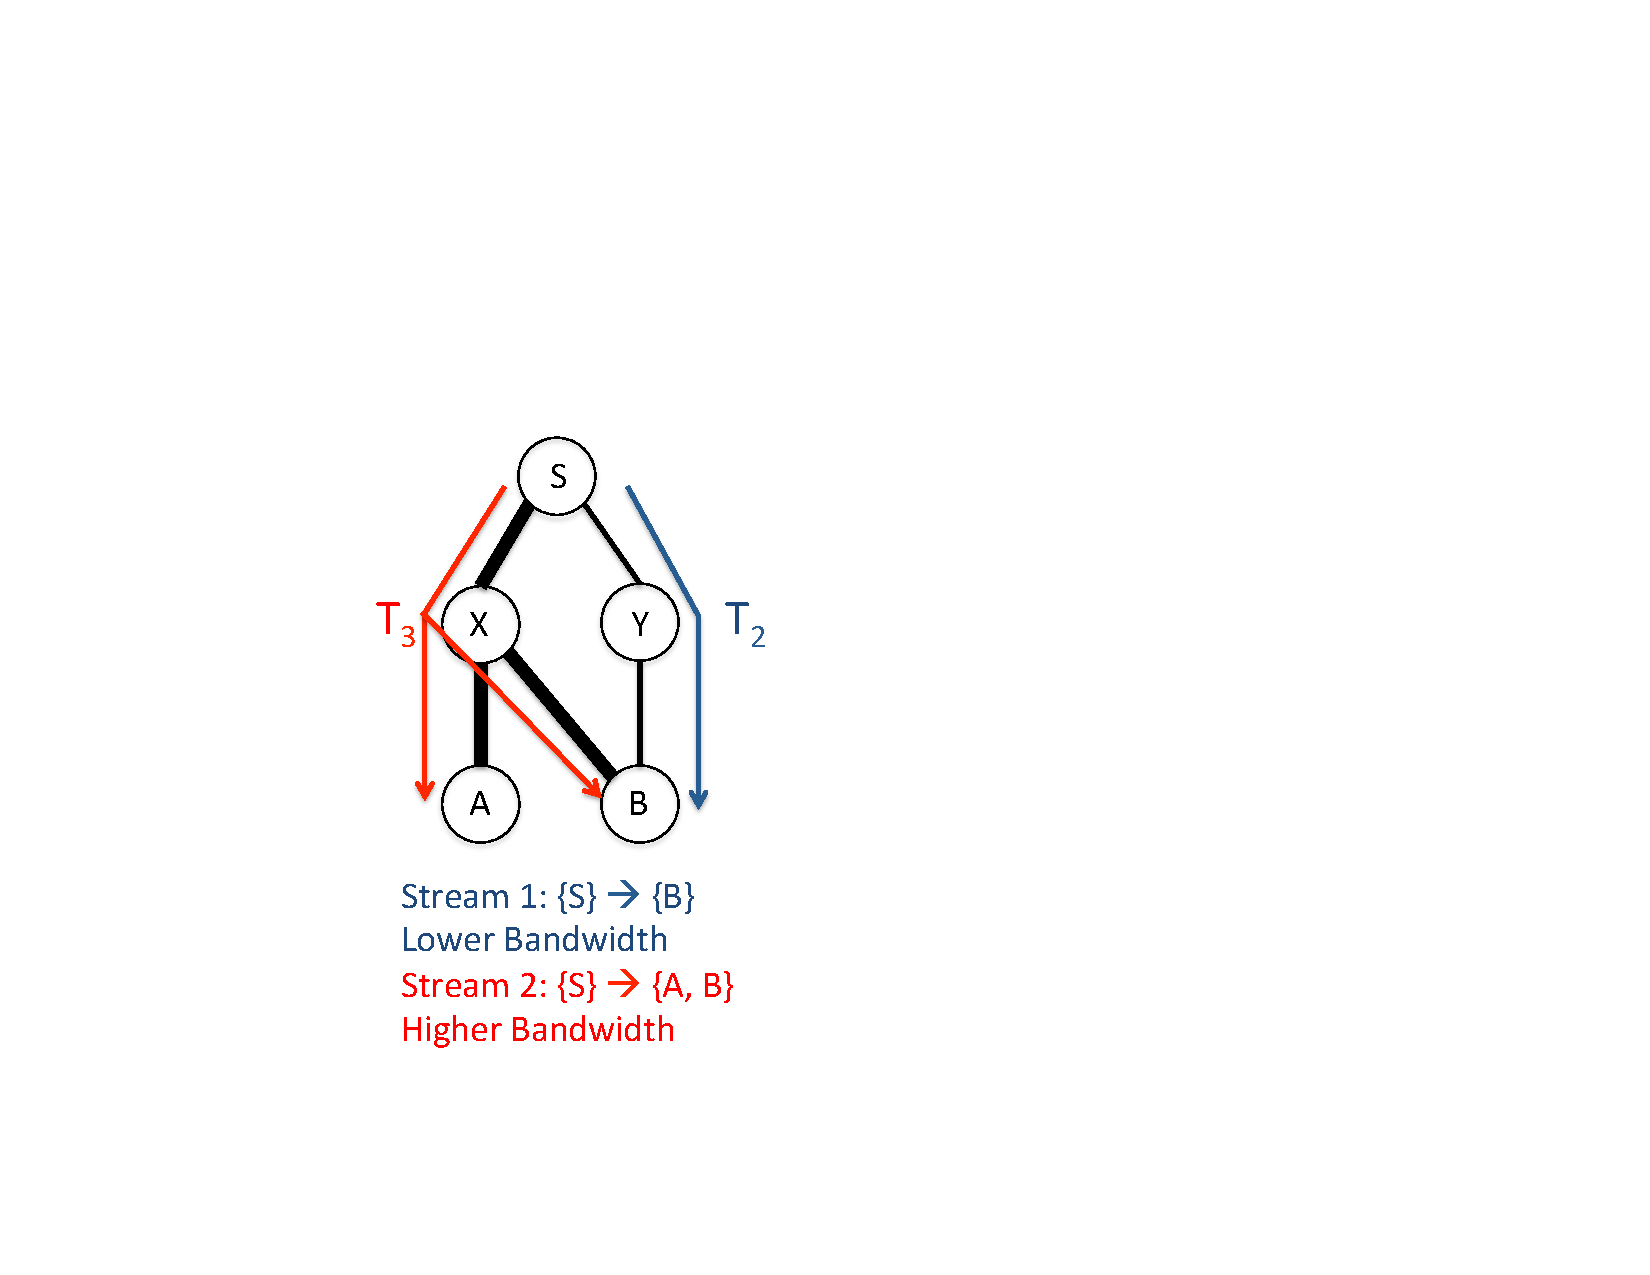
\includegraphics[scale=.40]{figures/toy}
  \caption{\\SDN+CDN}
  \label{fig:toy}
\end{minipage}
\end{figure}

\subsection{Current state-of-the-art}

Figure~\ref{fig:cdn} presents the high-level structure of a CDN's internal
video delivery system as described in ~\cite{akamai-live}. A set of co-located
servers form a cluster.
%Communication within the cluster can use multicast as it
%is often within a single LAN\@.  
Clients' video requests are directed to edge servers.  When an edge server gets
a request from a client, it subscribes to the content from one of the interior
clusters. The internal clusters are geo-distributed in well-provisioned
locations.  These servers directly receive content from the content sources (e.g., video origins).

The set of internal nodes are determined manually~\cite{akamai-live}, and thus
the distribution structure forms a rather rigid three-tiered hierarchy~\cite{spaa,akamai-live}.
Furthermore, the system does not have the knowledge of global resources, as distribution trees
are formed independently without much coordination.
For example, even though edge servers use multiple path from a content source
when the stream quality deteriorates, each edge server independently selects how many paths to use
without any coordination~\cite{akamai-live}.

\jc{need to define terminologies somehow: chunk, bitrate, stream, video server, origin}

\subsection{Why centralized control?}

Figure~\ref{fig:toy-alltrees} illustrates a simple example that 
demonstrates uncoordinated decision making leads to sub-optimal resource allocation. 
Links shown in bold are higher capacity than the non-bold links. 
%We wish to deliver two video streams (Stream 1 and Stream 2) through the network, both
%originating from source \emph{S}. 
There are two video streams (Stream 1 and 2) originating from source  \emph{S}.
The goal is to deliver Stream 1 to \emph{B} and Stream 2 to both \emph{A} and \emph{B}.

Three possible distribution trees exist in this configuration: $T_1$,
$T2$ and $T3$. 
Among the three only $T1$ and $T_2$ are useful for delivering Stream 1 to \emph{B}.
%However, $T_1$ provides higher bandwidth.
%$T_3$ is the only tree useful to Stream 2.
Now assume that the request for Stream 1 from B was made prior to the request
for the more popular Stream 2 (from \emph{A} and \emph{B}).

In a traditional CDN (Figure~\ref{fig:toy-current}), \emph{B} selects the interior node
(i.e. \emph{X} and \emph{Y}) to forward the request the content from based on some metric (e.g., network bandwidth). 
Thus, $T_1$ is chosen. When a request for Stream 2 arrives, $T_1$ is already occupying the link.
Therefore, either both Stream 1 and 2 suffers from poor quality or Stream 2 cannot be serviced. 

However, with coordination across streams, a better decision can
be reached as in Figure~\ref{fig:toy}.  To accommodate the more important request for Stream 2, 
the systems reduces the supported bitrates for Stream 1 and
serves it through $T2$.
%Although this selection means lower bandwidth for 
The overall bitrate available at each edge server is now much higher. 
Although this is a very simple example, the intuition is clear:
coordination of resource allocation can provide large benefits.


\subsection{Why not complete centralization?}


Our goal is to build a logically centralized architecture for CDNs. One approach towards this is to move all control and management logic to a physically centralized controller and only leave basic forwarding functionality in distributed data-plane nodes. The controller maintains an information base of network state, makes real-time decision and then disseminates the decision to each node in realtime. In addition, the controller is often replicated for fault tolerance, so it is required for multiple controllers to produce a consistent decision.
Such fully centralized architecture has been widely adopted in various IP-layer SDN systems for traffic engineering and enforcing routing policy in data center, enterprise network and WAN environment.
At a first glance, it is natural to employ the same centralization scheme to for CDNs. However, a careful revisit of the overheads and the realities in CDN environment shows that a fully centralized control plane is not as practical as in IP layer and instead, a partial centralized system will serve better under the constraints in CDN environment. 

A complete centralized control plane introduces delay, places cost to achieve consistency on the controllers, and thus limits system's scalability in terms of the number of events that it can handle efficiently. These overheads will only be exaggerated in large-scale overlay systems like CDNs. 
%We examine these overheads in CDN environments to show that fully centralized design cannot meet the needs of CDN control plane.

\begin{packeditemize}
	\item {\bf Propagation delay} The propagation delay results from the inherent latency between the controller and servers in data plane. It includes collection delay, i.e., the time between network states change and the controller is aware of the change, and dissemination delay, i.e., the time between controller makes decision and the decision is fully applied by the servers. \jc{Provide some evidence...}
%The propagation delay poses the lower bound of controller's response time after a network state change. To examine how much impact the propagation delay has on control plane response time in CDNs, we show... \jc{Real data to show propagation delay (statistics collection and decision dissemination delay) in overlay network is far larger than in that in data center networks or inter-DC WAN}
	\item {\bf Multiple controller consistency} To be robust to network partitions and avoid creating a single point of failure, the controller should be replicated and locate in different geo-locations. However, replication introduces the possibility that each controller replica may have different views of the network state and thus make different decisions. \jc{Provide some evidence...}
%Our analysis using \fillme data show that to to achieve consistency among these geo-distributed controllers using traditional consensus protocols(e.g., Paxos) could be time-consuming. \jc{Real data to show the overhead to achieve Paxos consensus among geo-distributed controllers is untolerable.}
\end{packeditemize}

\jc{is it fair to say CDN needs to manage more nodes than traditional SDN?}

Despite of these exaggerated overheads, CDNs at the mean time also provide two unique opportunities in its data plane -- software-controlled servers and flexible forwarding semantics -- that we can leverage to reduce the overheads by delegating some tasks away from the controller.
\begin{packeditemize}
	\item {\bf Software-controlled servers} Unlike in IP layer where switches and routers are specialized, hardware-controlled and costly to update, CDN data plane consists of servers that run software on general-purpose machines. Thus, frequent update on the software to control the data-plane behavior can be done with far less overhead than in switches or routers. 
	\item {\bf Flexible forwarding semantics} Forwarding semantics in content delivery is content-oriented and is different to packet or flow-based forwarding which is location-based. For example, content can be pushed, pulled, or cached locally. Each video is also encoded in multiple bitrates and can be also obtained from multiple sources. Moreover, today's CDN servers often have flexible request forwarding strategies that include loop detection, multi-path for load balance and simple policy-awareness (e.g., middlebox traversal) as basic functions. Therefore, it is redundant to re-implement these logics at the controllers.
\end{packeditemize}

%(move these to related work) To handle such scalability issues, serial optimization has been proposed. DevoFlow allows rules to be prefetched and cloned to the switches in advance. Onix supports a hierarchy between controllers and allows aggregation of information along the hierarchy. Kandoo allows parts of the controller application's logic to be run inside local controllers that are closer to the switches.


\subsection{Our approach: partial centralization}

While there are incremental fixes proposed to reduce overheads (e.g., \cite{DevoFlow, Onix, Kandoo}, etc) of complete centralization, we explore another design option that can greatly simplify the control plane by leveraging the flexibility of CDN data plane. 
Instead of enforcing real-timeness and consistency on the controllers, we relax these constraints, push consistency control and real-time adaptation to software on the distributed node, and leave only global optimization in the controllers.
The philosophy behind this design choice is that, for wide-area overlay networks like CDNs, it is best to {\it simplify the controller} (i.e., leaving only works that involve global knowledge in the controller) rather than to {\it simplify the data plane} (i.e., pushing all works except forwarding to the controller).


\begin{figure}[h!]
\centering
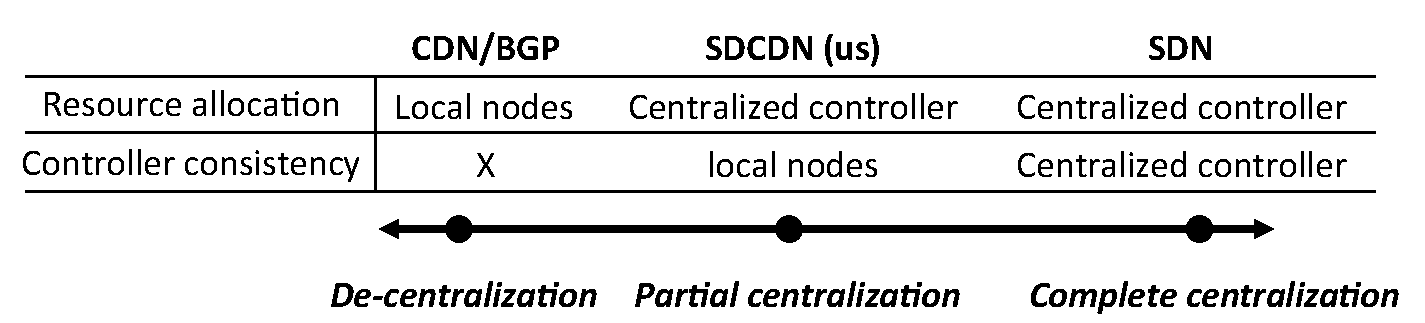
\includegraphics[width=1.0\columnwidth]{figures/design-space-3.pdf}
\caption{Design choices}
\label{fig:design-space}
\end{figure}


Figure~\ref{fig:design-space} compares the different design choices of SDN (e.g., Onix), CDN, and \SDCDN in two dimensions, i.e., resource allocation and consistency control. Unlike SDN or current CDNs which completely rely on local or centralized decision, SDCDN performs these functionalities in both controller and distributed servers.

	\myparatight{Resource allocation} Since the centralized controller is not sufficient for real-time decision, the resource allocation in SDCDN is done in two time scales. The controller performs global coordination with less constraints on real-timeness and produces {\it hint}s to each server. The local control process performs real-time resource allocation (e.g., path selection) based on the hints of global control process. Therefore, the hints and real-time use of them becomes critical in balancing the global optimality and responsiveness in real time (as discussed in Section~\ref{?}).

	\myparatight{Controller inconsistency} We let multiple controllers (i.e., global control processes) make decisions independently, and each server will receive multiple and possibly inconsistent decisions of controllers. SDCDN relies on servers to resolve the inconsistency if it exists, and merge them into a final decision used by data plane. Therefore, it is critical merge these decisions in a fashion that more fresh decisions are preferred but with less instability (as discussed in Section~\ref{?}).

Figure~\ref{fig:design-space} also depicts the spectrum of design space from de-centralization to complete centralization.  When projecting related systems onto this spectrum, current CDNs and SDNs are closer to the decentralization and centralization end respectively, and our design of SDCDN is in the middle of what we call {\it partial centralization}.
Although the concept of partial centralization of system design itself is not an innovation and it has been used for years (e.g., \cite{?}), our contribution is to exploit its potential benefits in implementing a control plane for wide-area overlay networks through a customized design in CDN environments.







